\chapter{Must Have Concepts}
During this chapter, we're going to discuss topics that help understand the technology developments made along the thesis project.

\section{The IOb-SoC Template}
\label{section:the_iob_soc_template}

\begin{figure}[!h]
    \centering
    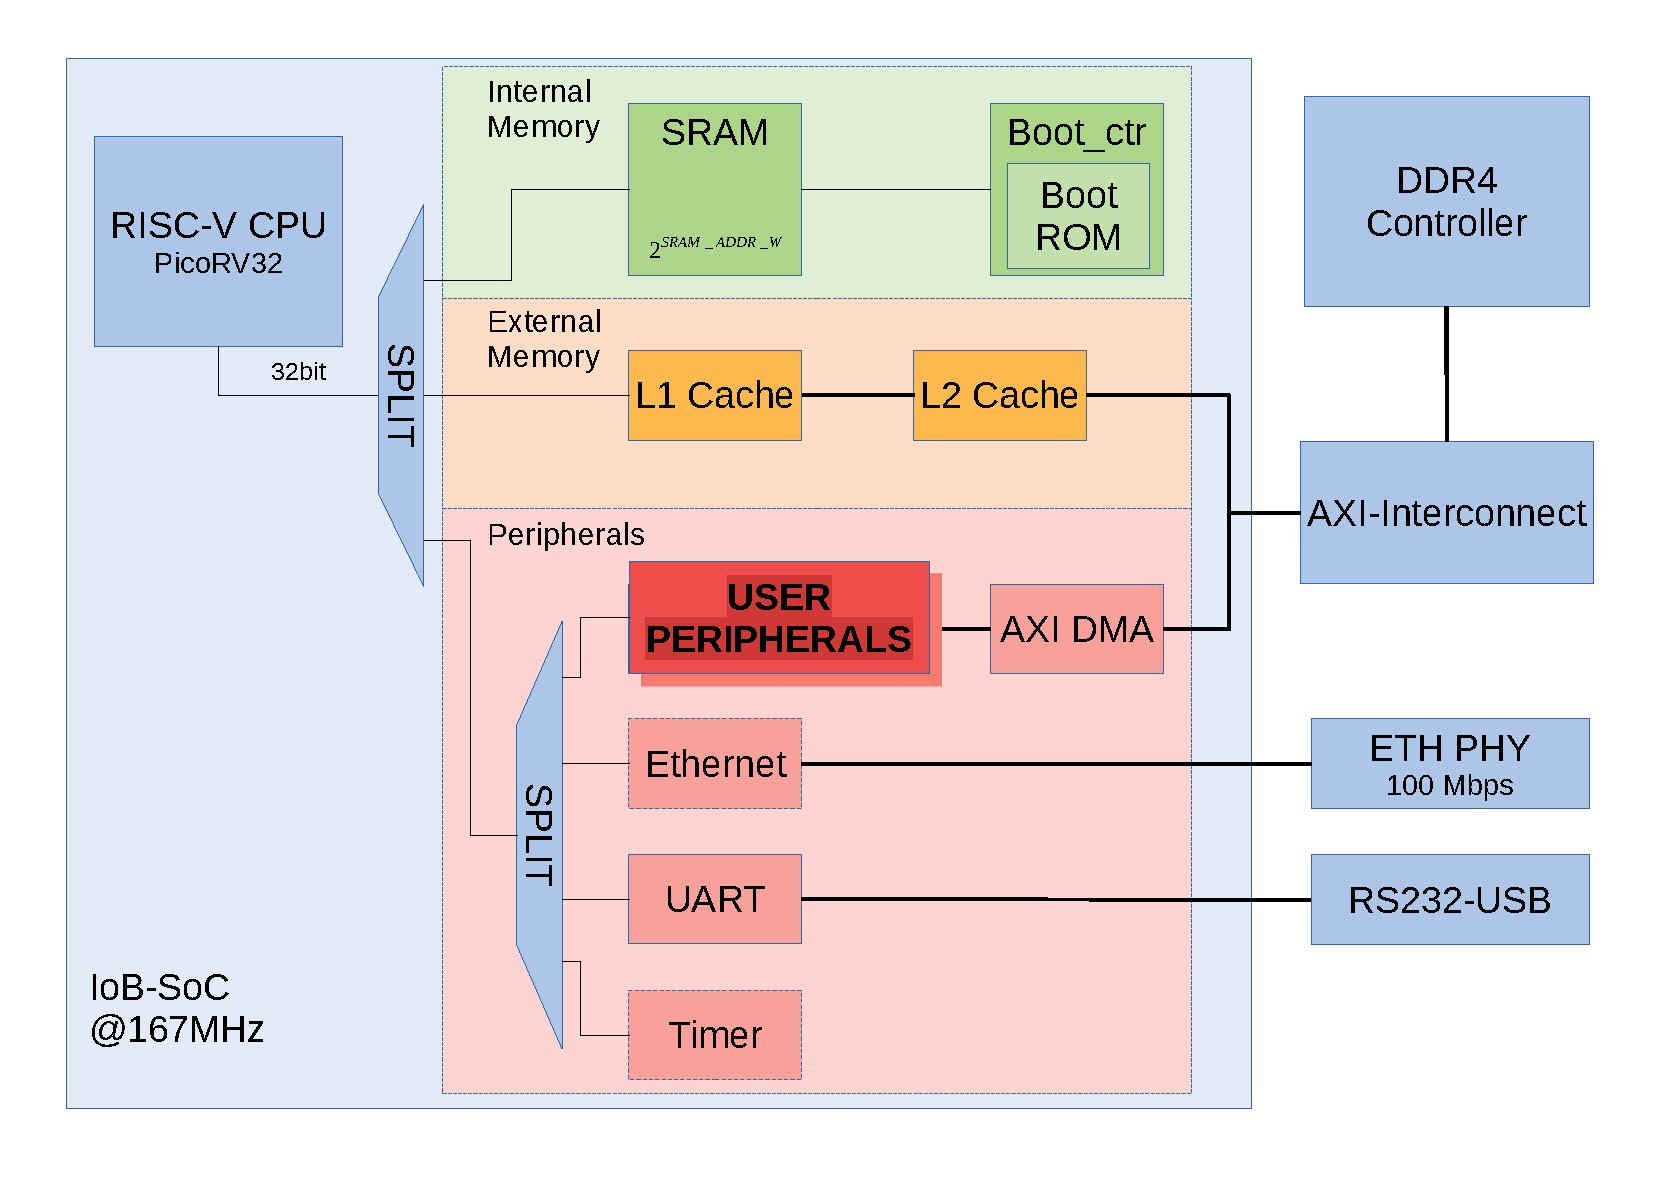
\includegraphics[width=0.7\linewidth]{bd_original.pdf}
    \caption{\textit{IOb-SoC} sketch.}
    \label{fig:bd_original}
\end{figure}

\subsection{Adding peripherals}
\subsection{Internal Buses}
Review the \enquote{cpu\_i\_resp}, \enquote{cpu\_d\_resp}, \enquote{cpu\_i\_req} and \enquote{cpu\_d\_req} signals.

\subsection{\textit{iob-split} and \textit{iob-merge}}
The \textbf{\textit{iob-split}} is simply a configurable \acrfull{demux}. Meaning that when the \textit{iob-split} hardware module is instantiated the developer can configure it. The developer is able to change the size of the \acrlong{demux} and the selection bits, through N\_SLAVES and P\_SLAVES respectively. N\_SLAVES corresponds to the number of slaves, witch can also be seen as the number of the \acrshort{demux} outputs. P\_SLAVES indicates the slave select word \acrfull{msb} position, in other words it is the position of the \acrshort{msb} of the \acrlong{demux} selection bits. The number of the selection bits is given by equation \ref{eq:number_bits}.

\begin{equation}
    \label{eq:number_bits}
    Nb = log_2(N\_SLAVES)+(log_2(N\_SLAVES)==0)
\end{equation}

The \textbf{\textit{iob-merge}} works similar to the \textit{iob-split} but instead of being a \acrshort{demux} it is a configurable \acrfull{mux}. Meaning that instead of having multiple outputs and one input it has multiple inputs and one output. The number of inputs is indicated by N\_SLAVES and the selection bits are chosen by P\_SLAVES.

\subsection{Bootloader and bare-metal firmware}

\section{Open Source Verification tools}
For testing purposes, it is important to have a good hardware simulation environment. For that, we take advantage of already existing and well-developed tools. There exist a number of simulation tools, most of them are proprietary, as for example \textit{'xcelium'} from \textit{'Candence'}. Its utilization can increase the cost of a project significantly. In this Thesis we will make an effort of using open-source, free to use, verification tools. In specific, we will take advantage of \textit{'Icarus Verilog'} and \textit{'Verilator'}. Although both tools are for verification, they serve different purposes, due to their characteristics.

\begin{itemize}
    \item \textbf{\textit{'Icarus Verilog'}} is a Logic Simulator that uses verilog or system-verilog testbenchs to test the UUT (Unit Under Test). Unfortunately, its support for system-verilog is limited and some designs might not run in this simulator. \textit{'Icarus Verilog'} is also known as \textit{'IVerilog'}.
    
    After compiling the hardware design, \textit{'IVerilog'} outputs a file which can be run line by line to simulate designed logic.
    
    \item \textbf{\textit{'Verilator'}}
\end{itemize}

\textbf{The biggest differences} are: \textit{'Verilator'} only represents logic signal as 1's or 0's, contrary to \textit{'IVerilog'} which also represents unknown values as X's; Since \textit{'Verilator'} ends up being a C++ program it is much faster to run the simulation than with \textit{'IVerilog'}; On another perspective \textit{'Verilator'} is slower than \textit{'IVerilog'} to interpret the hardware logic design.
As such, it is easier to use \textit{'IVerilog'} to detect errors on the design, but it is better to use \textit{'Verilator'} for more complexed simulations.

\subsection{Qemu Simulation}
https://www.sifive.com/blog/risc-v-qemu-part-1-privileged-isa-hifive1-virtio

\section{RISC-V}
Talk about the 32 registers in the register file

The instruction each ISA extension contains...

\acrfull{csr} needed to run a full feature OS...

The RISC-V \textbf{CLINT} is described ...
Platform must support an ACLINT MTIME counter resolution of 100ns or less (corresponding to a clock tick frequency of at least 10 MHz).

The RISC-V \textbf{PLIC} was first described in the privilege instructions documentation, but since version 1.10 it was moved to its own document.

\section{RISC-V UART/Serial Console}
In the RISC-V Platform Specification~\cite{riscv_platform_specification} it is defined that every embedded \acrfull{os} is required to have a \acrshort{uart} port implementation that is register-compatible with the industry standard \textit{UART 16550}, which was studied in chapter~\ref{section:uart16550}. The \textit{UART 16550} already exists for a long time, it was released by \textit{National Semiconductor} in 1987, and is present and supported by a large number of software and hardware. The \textit{UART 16550} is often used connected to an RS-232 interface and in this project the development boards used are connected through RS-232 to the computer.

The \textit{UART 16550} registers are...

\section{The Linux Boot Flow}
\subsection{Bootloader firmware}
\subsection{What is a device tree?}


